\newpage
\chapter{PLANIFICACIÓN Y GESTIÓN DEL TFG}
\newpage

\newpage
\section{PLANIFICACIÓN DEL PROYECTO}

\subsection{Identificación de Interesados}
\begin{itemize}
\item \textbf{Usuarios de la aplicación web del museo}: Personas interesadas en la información ofrecida de las piezas expuestas en el museo que consultarán la página web.
\item \textbf{Tutor de este trabajo y administrador del museo}: Persona que ha propuesto el proyecto de digitalización del museo, y que lo administrará una vez terminado el desarrollo.
\item \textbf{Autora del trabajo y desarrolladora}: Encargada del desarrollo de la aplicación y de la documentación asociada.
\end{itemize}


\subsection{%OBS y 
PBS}
\begin{figure}[H]
\centering
\centerline{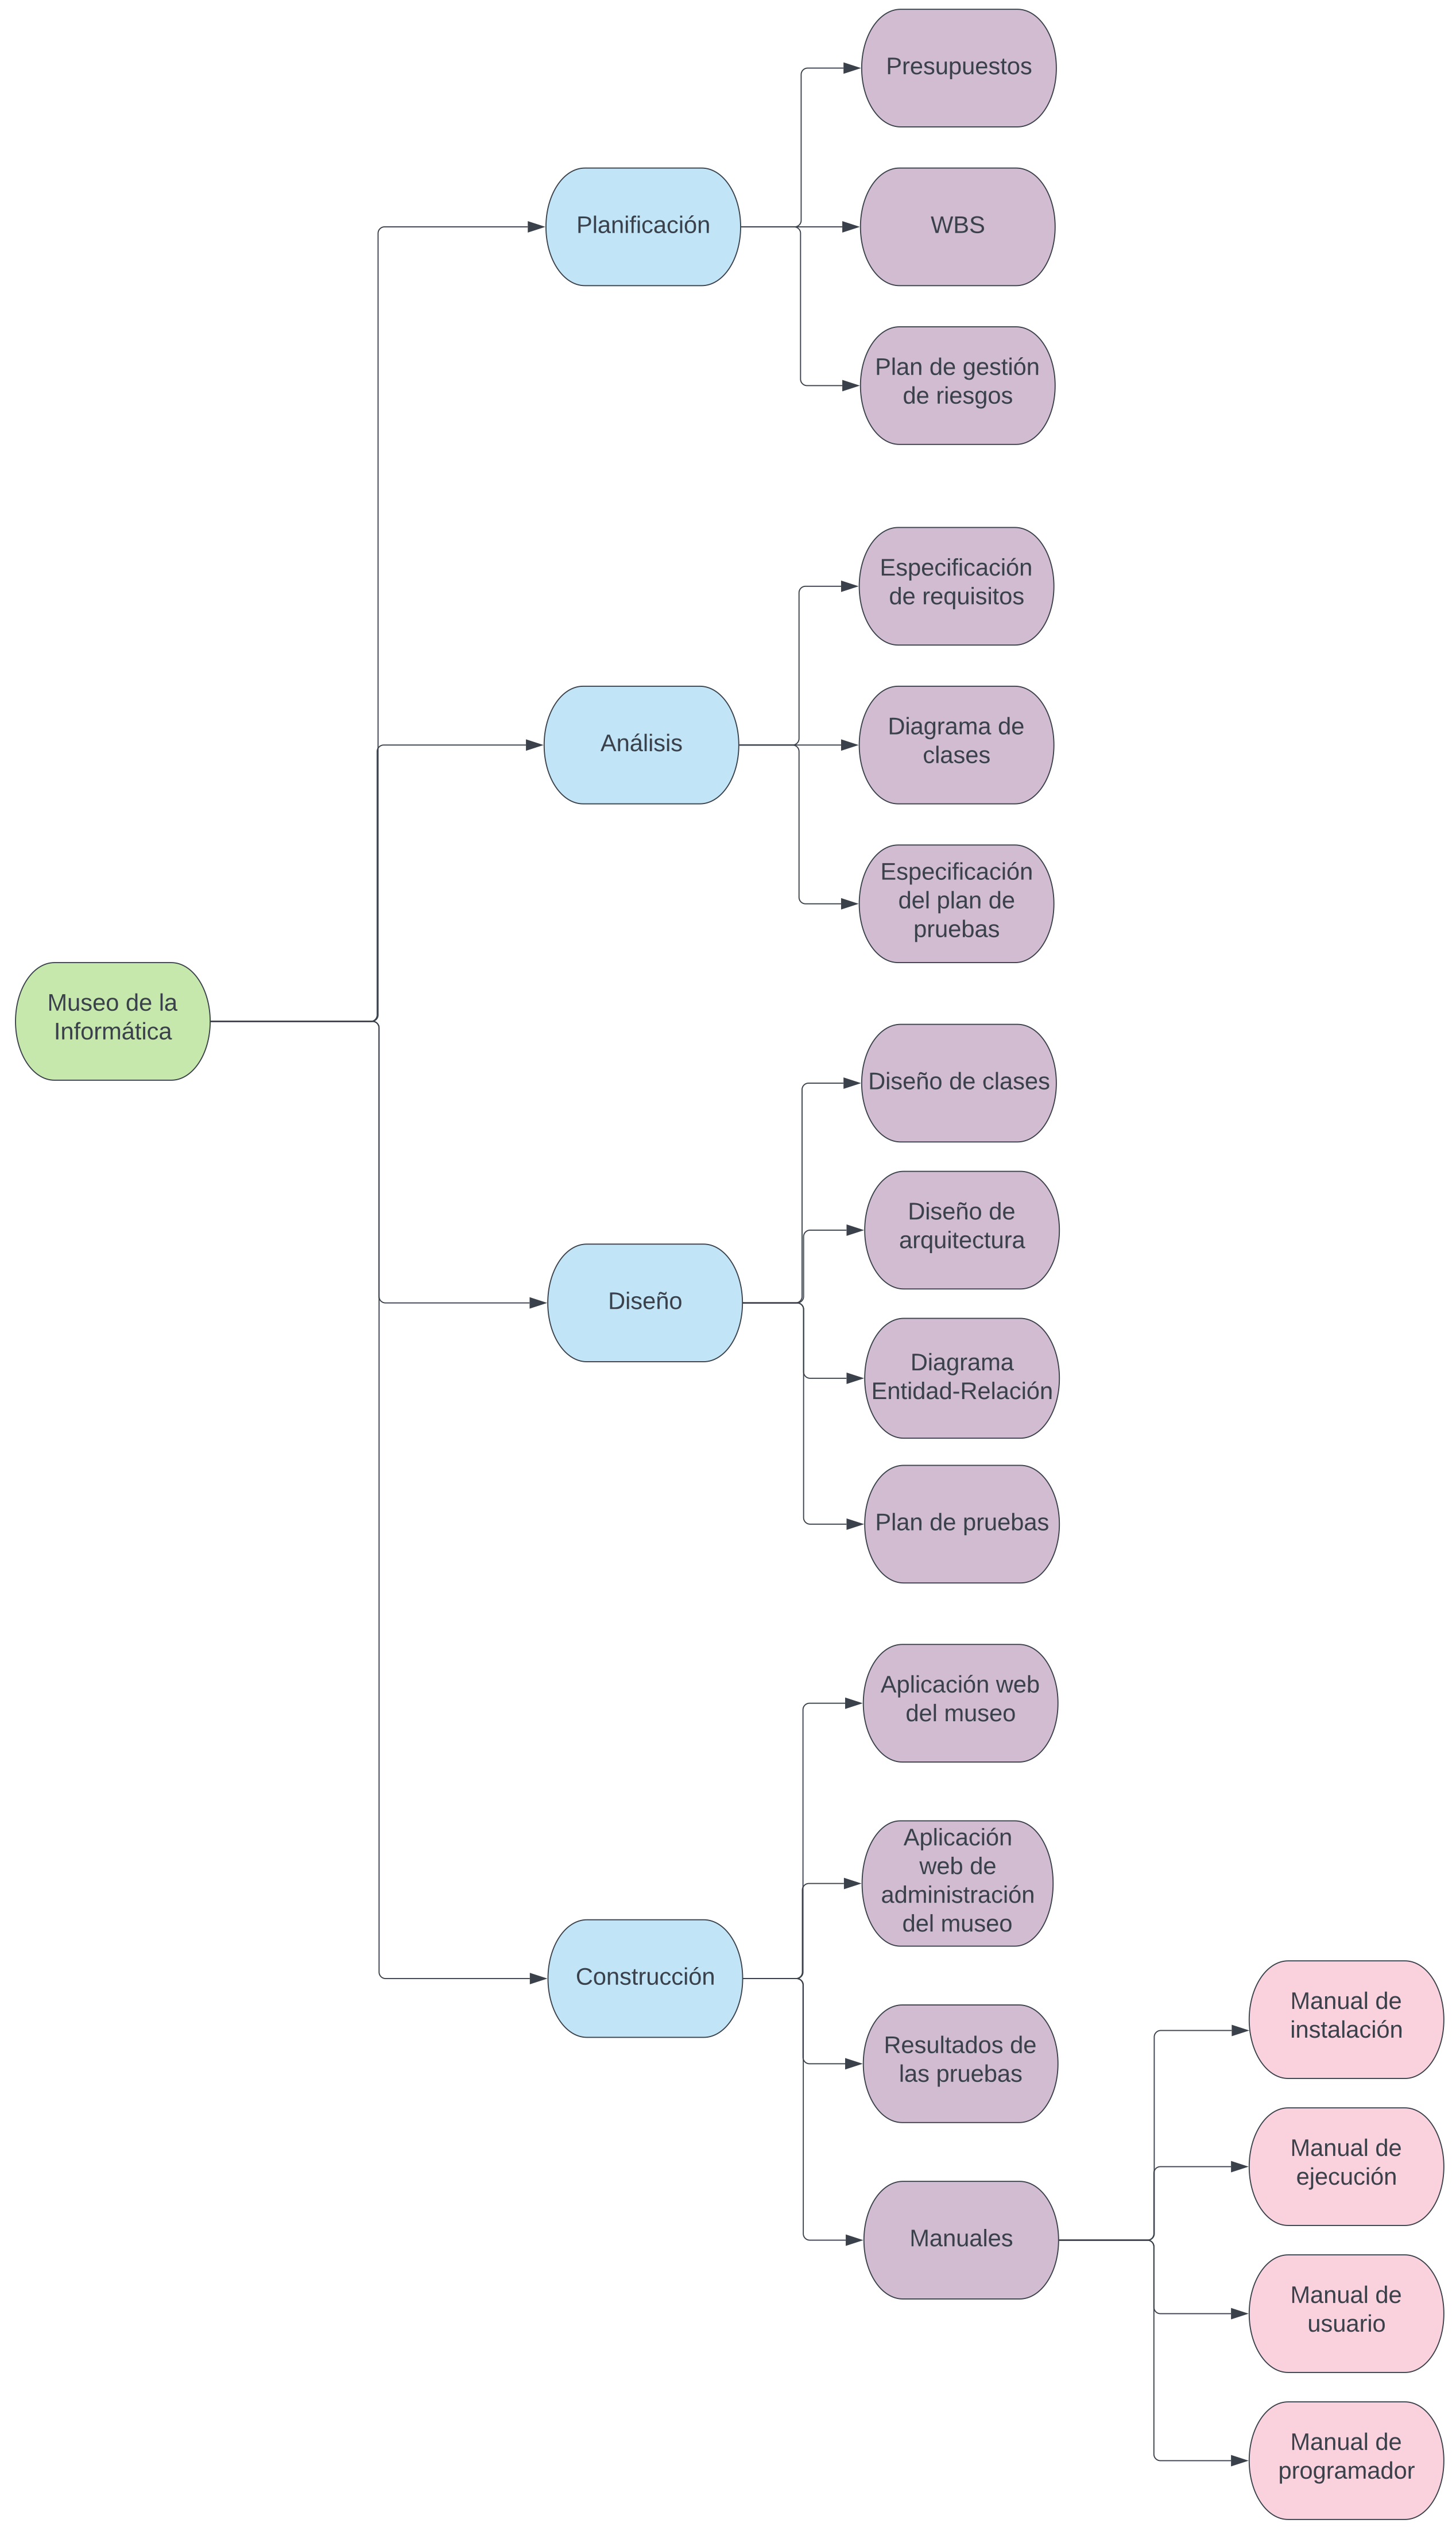
\includegraphics[scale=0.25]{PBS}}
\caption{Product Breakdown Structure}
\end{figure}


\subsection{Planificación Inicial. WBS}
A continuación se muestra la planificación inicial del proyecto y el correspondiente diagrama de Gantt. Para visualizar mejor esta planificación se adjunta el archivo \textit{WBS.mpp} como se especifica en la sección \ref{sec:contenido_anexos}. Se han planificado jornadas de trabajo de 3 horas diarias, y la estimación de la duración total del proyecto es de 258 horas.
\begin{landscape}
\pagestyle{empty}
\begin{figure}[H]
\centering
\centerline{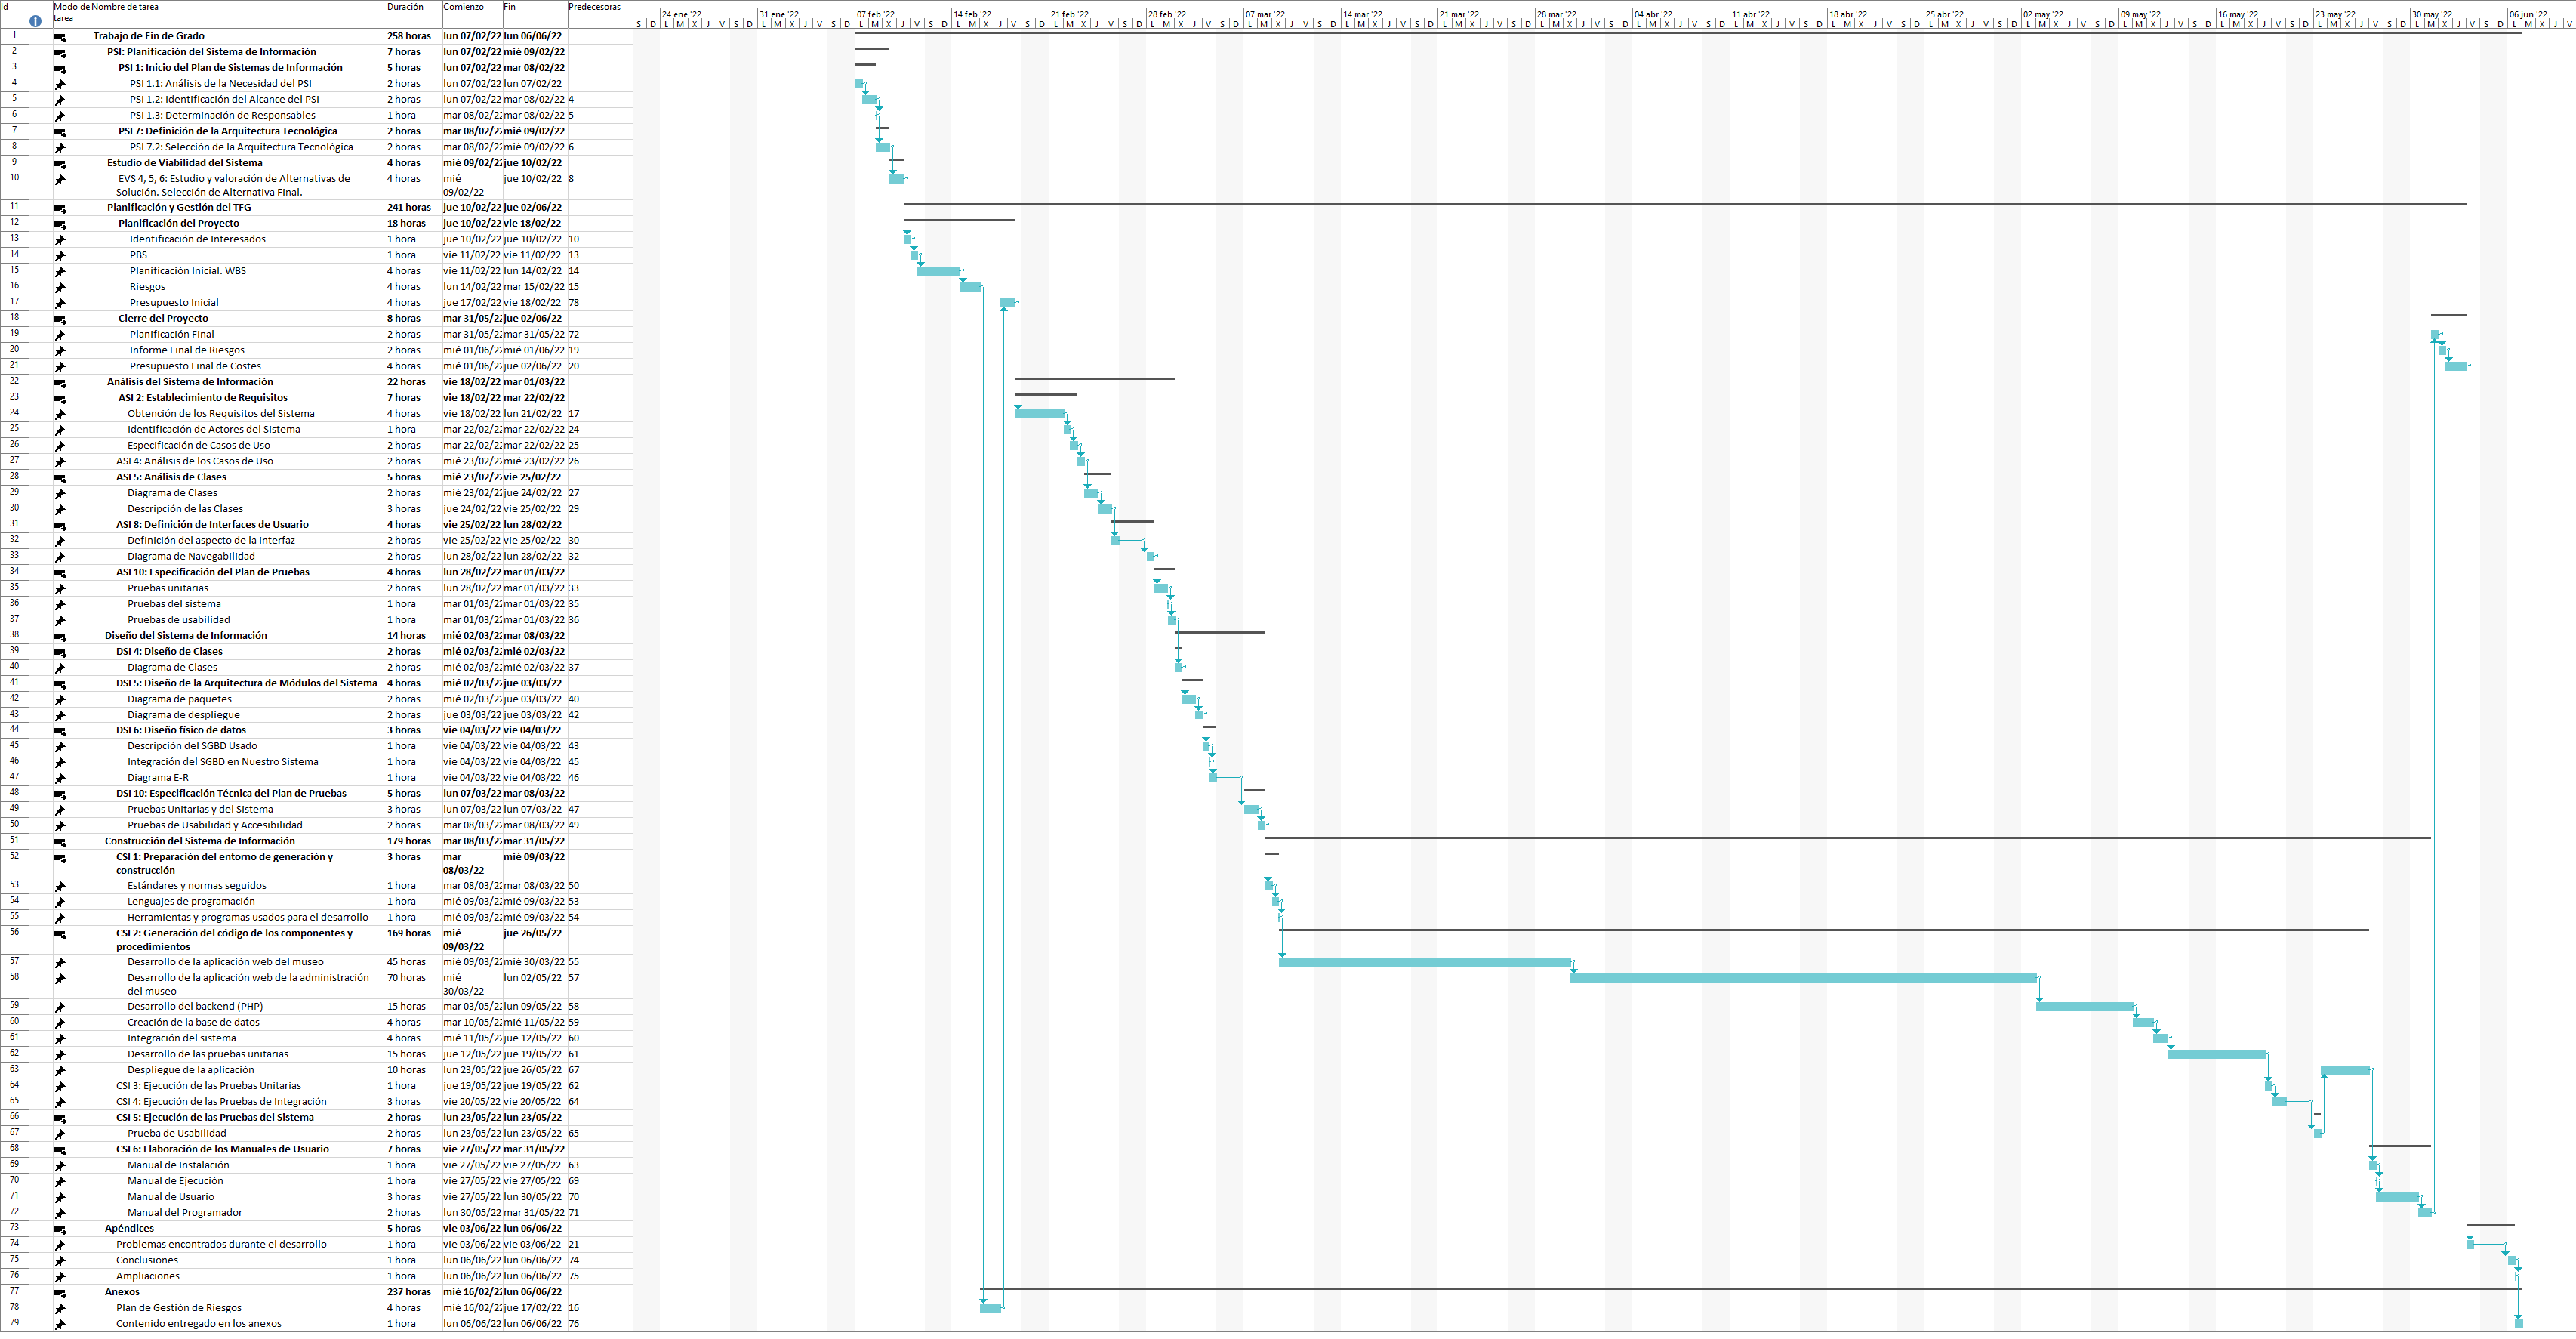
\includegraphics[scale=0.3]{plan-inicial}}
\caption{Planificación inicial, diagrama de Gantt}
\end{figure}

\end{landscape}
\pagestyle{fancy}
\subsection{Riesgos}\label{sec:riesgos}

\subsubsection{Plan de Gestión de Riesgos} 
El plan de gestión de riesgos del proyecto se define en el anexo \ref{sec:plan-riesgos}.

\subsubsection{Identificación de Riesgos}
Se han identificado un total de siete riesgos:
\begin{enumerate}
\item Las tareas tienen una duración mayor a la planificada inicialmente.
\item Equivocación a la hora de entender un requisito.
\item El ordenador del desarrollador deja de funcionar.
\item El servidor deja de funcionar.
\item Fallo en la aplicación al pasar a producción.
\item Adición de un segundo servidor.
\item Problemas de comunicación con el tutor del proyecto.
\end{enumerate}

\subsubsection{Registro de Riesgos} 
A continuación se muestran los riesgos identificados, priorizados según su probabilidad e impacto. De cada riesgo se especifica categoría, probabilidad, impacto, prioridad y estrategia a seguir. Esta tabla se encuentra en el archivo adjunto \textit{Informe\_Riesgos.xlsx}.
\begin{figure}[H]
\centering
\centerline{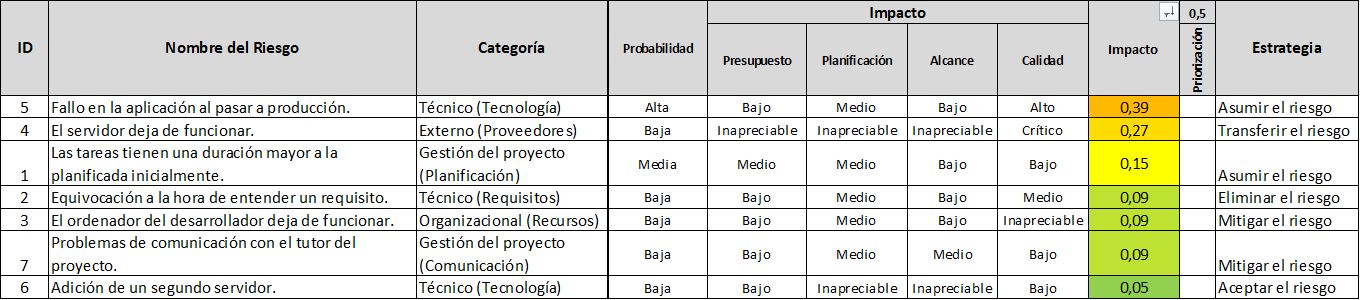
\includegraphics[scale=0.55]{riesgos}}
\caption{Registro de riesgos}
\end{figure}

\subsection{Presupuesto Inicial}
En esta sección se muestran los presupuestos de costes y de cliente realizados en base a la planificación inicial del proyecto. Estas tablas con sus pertinentes cálculos se encuentran en el archivo adjunto \textit{Presupuesto inicial.xlsx}.
\subsubsection{Presupuesto de Costes}
\begin{figure}[H]
\centering
\centerline{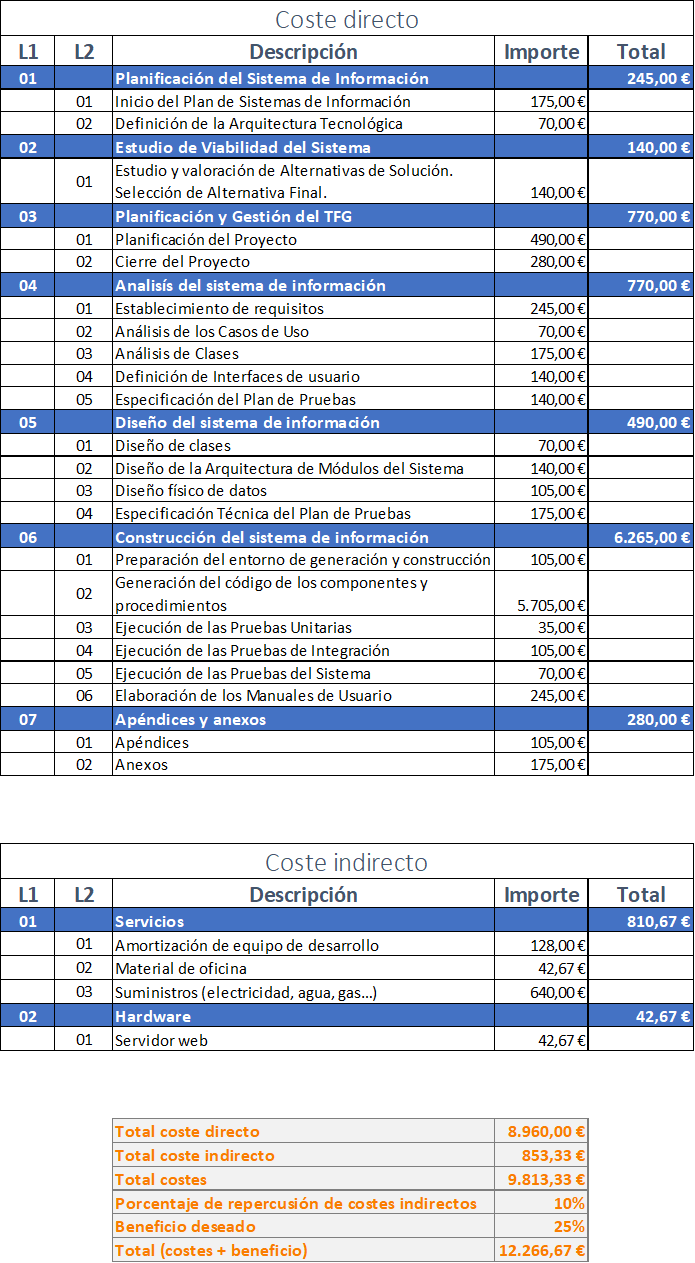
\includegraphics[scale=0.6]{presupuesto-costes-inicial}}
\caption{Presupuesto Inicial de Costes}
\end{figure} 

\subsubsection{Presupuesto de Cliente} 
\begin{figure}[H]
\centering
\centerline{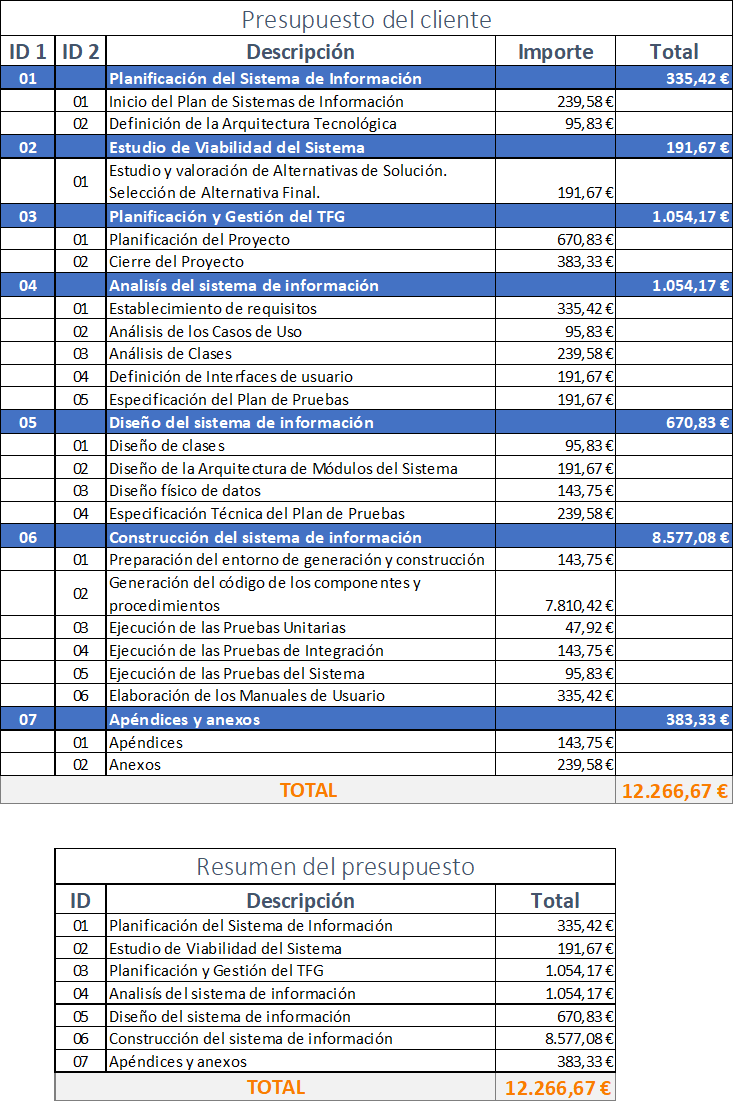
\includegraphics[scale=0.6]{presupuesto-cliente-inicial}}
\caption{Presupuesto Inicial de Cliente}
\end{figure} 


%\newpage
%\section{EJECUCIÓN DEL PROYECTO}
%
%\subsection{Plan Seguimiento de Planificación}
%
%\subsection{Bitácora de Incidencias del Proyecto}
%
%\subsection{Riesgos}


\newpage
\section{CIERRE DEL PROYECTO}

\subsection{Planificación Final}
A continuación se muestran las horas de trabajo realizadas finalmente (columna \textit{Trabajo}) en comparación con las planificadas. Esto se incluye también en el archivo adjunto \textit{WBS.mpp}. La duración final del proyecto ha sido de 291.25 horas, 33.5 horas más que las iniciales.
\newpage
\pagestyle{empty}
\begin{figure}[H]
\vspace{-25mm}
\centering
\centerline{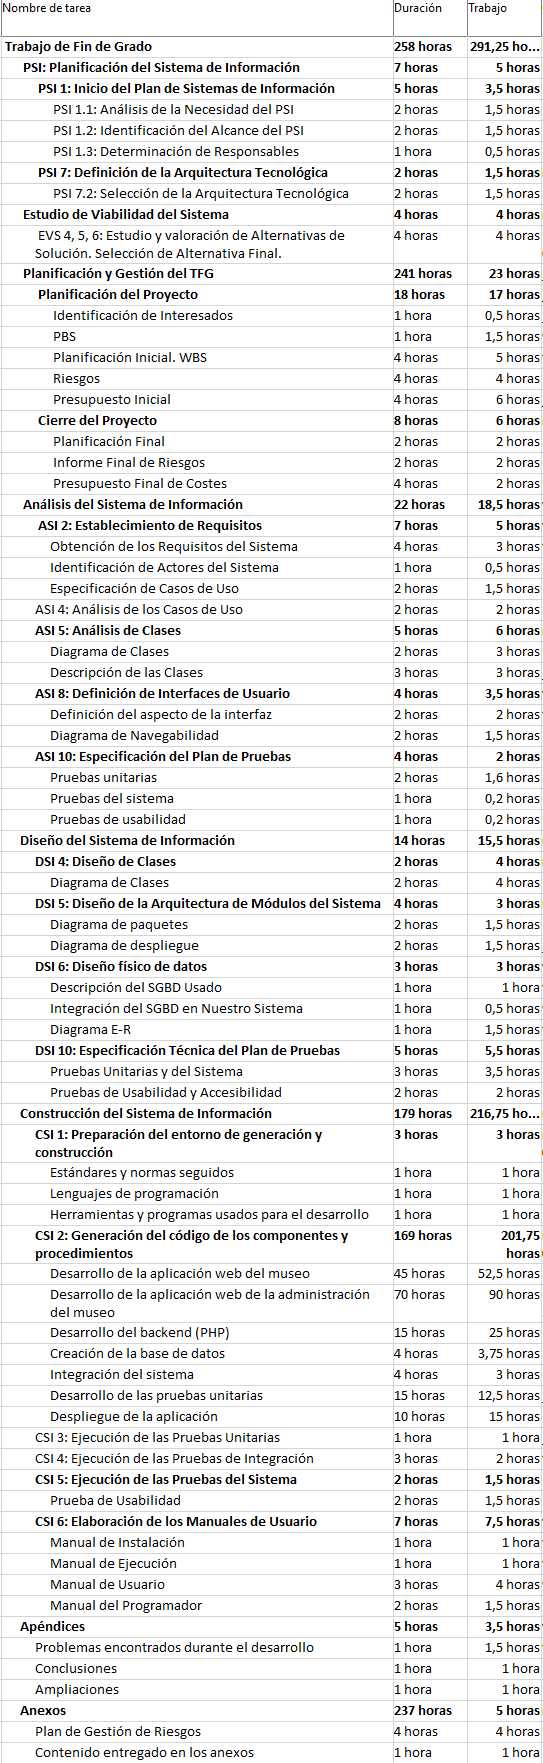
\includegraphics[scale=0.55]{plan-final}}
\caption{Planificación final}
\end{figure} 
\newpage
\pagestyle{fancy}
\subsection{Informe Final de Riesgos}
En esta sección se describirán los riesgos del proyecto que se identificaron en la sección \ref{sec:riesgos} y que finalmente ocurrieron.
\begin{itemize}
\item \textbf{Fallo en la aplicación al pasar a producción.} Una vez terminadas las aplicaciones, pasando con éxito las pruebas unitarias y funcionando correctamente en el entorno local, se desplegaron en el servidor. Al probarlas una vez desplegadas ocurrieron errores con las rutas de la aplicación, que aunque no daban problema en local, no tenían la configuración adecuada para funcionar en producción. Identificar cuál era el error y corregirlo hizo que el despliegue de la aplicación tuviera una duración mayor a la estimada.
\item \textbf{Las tareas tienen una duración mayor a la planificada inicialmente.} Las estimaciones realizadas en un principio fueron más o menos acertadas para las tareas de documentación, pero se quedaron muy cortas en el desarrollo de las aplicaciones, ya que el tiempo dedicado a aprender sobre las tecnologías utilizadas y a corregir fallos cometidos durante la programación, aunque se había tenido en cuenta al hacer la planificación, fue superior al esperado.\par  Esto ha repercutido en el plazo de entrega (hubo que retrasar la entrega a la convocatoria extraordinaria de julio) y en los costes del proyecto, ya que como se podrá ver en el siguiente apartado, el total del presupuesto final de costes es superior al calculado inicialmente debido a las horas trabajadas no planificadas.
\end{itemize}
\subsection{Presupuesto Final de Costes}
A continuación se muestra el presupuesto final de costes del proyecto. Se puede observar que el importe total de los costes es mayor al calculado en el presupuesto inicial (1351€ más), debido a que las horas de trabajo realizadas han sido superiores a las planificadas inicialmente. Estas tablas también se adjuntan en el archivo \textit{Presupuesto final.xlsx}.
\begin{figure}[H]
\centering
\centerline{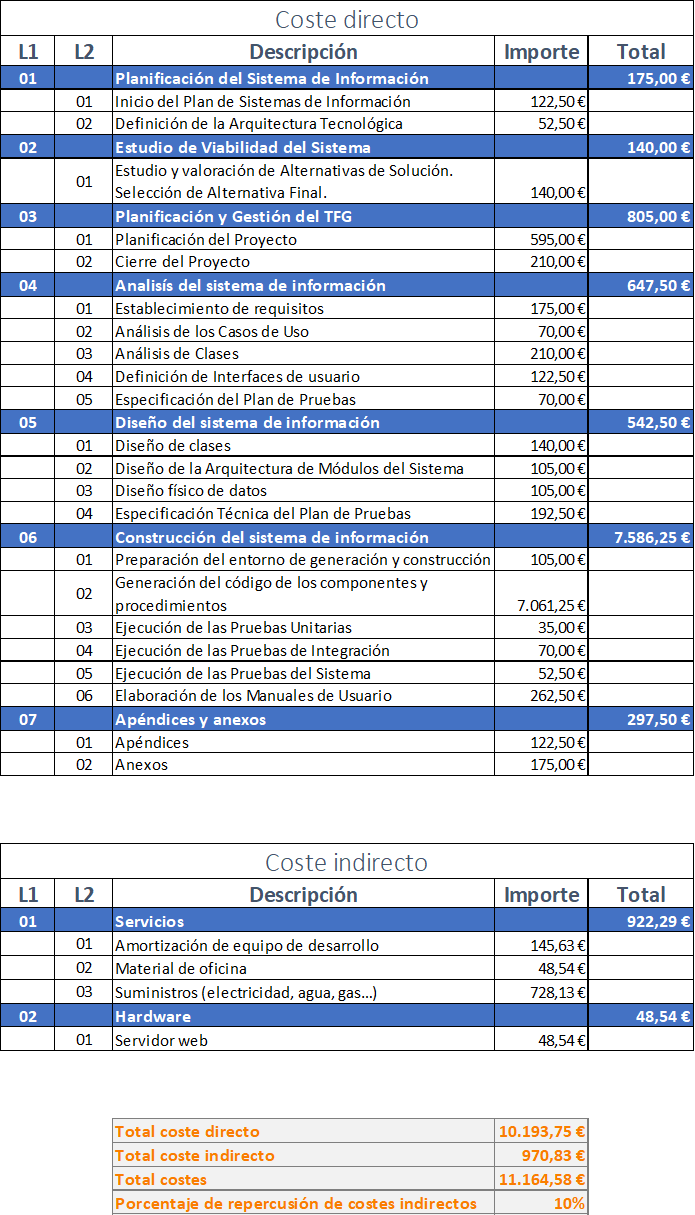
\includegraphics[scale=0.6]{presupuesto-costes-fina}}
\caption{Presupuesto Final de Costes}
\end{figure} 

%\subsection{Informe de Lecciones Aprendidas}
